\documentclass{article}
\usepackage{booktabs}
\usepackage{tabularx}
\usepackage{float}
\usepackage{graphicx}
\usepackage{geometry}
\geometry{margin=1in}
\begin{document}

\section*{Moda de evaluaciones no RAG}

\begin{table}[H]
\centering
\caption{Valor más frecuente (moda) por campo de evaluación}
\begin{tabularx}{0.6\textwidth}{lX}
\toprule
\textbf{Campo} & \textbf{Valor más frecuente} \\
\midrule
Relevancia & alta \\
Claridad & alta \\
Coherencia & alta \\
\bottomrule
\end{tabularx}
\end{table}

\begin{figure}[H]
\centering
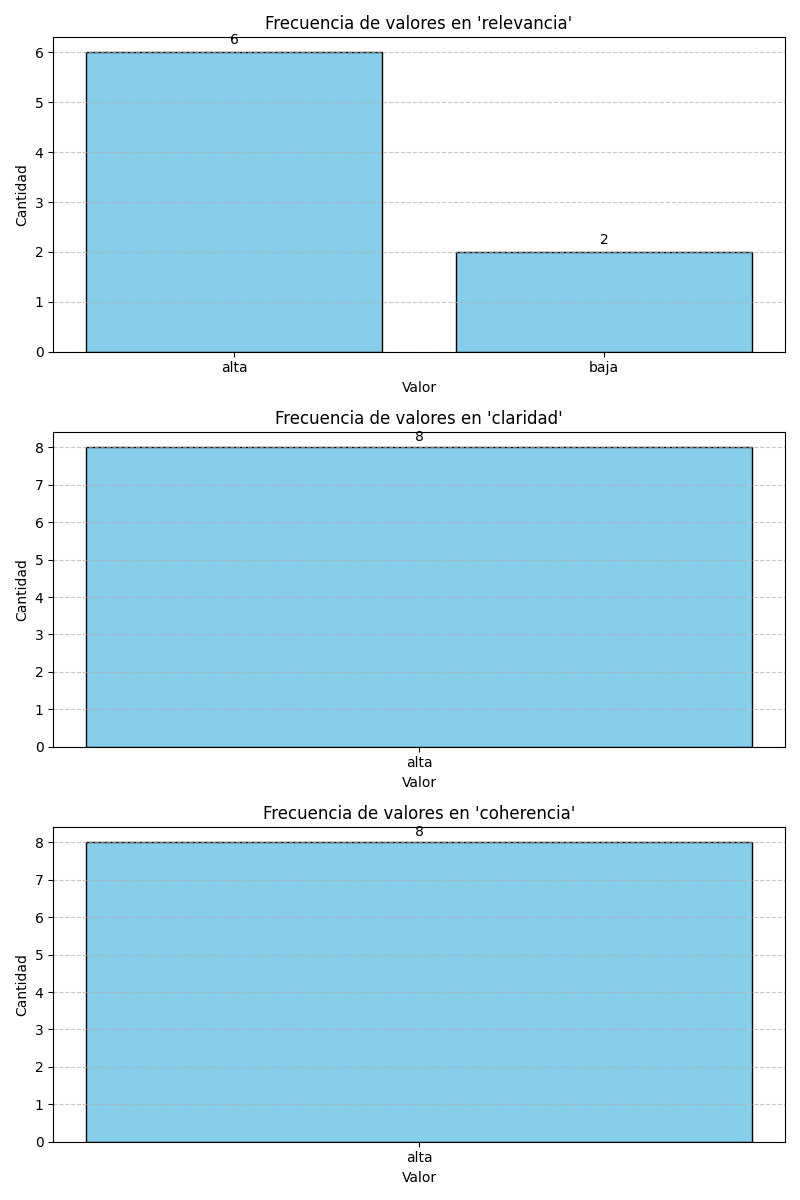
\includegraphics[width=0.8\textwidth]{../graficos/no_rag_frecuencias.png}
\caption{Frecuencia de valores por campo de evaluación}
\end{figure}

\end{document}
